\section{Evaluation Protocol}
As mentioned earlier our evaluation protocol focuses on the absolute evaluation of the 48 stories on each of the 14 questions shown in Table \ref{CreativityTest} as well as a relative evaluation of 12 clusters for discerning whether a story on the same plot within an individual cluster has been produced by a human or an LLM( Turing Test).
\subsection{Absolute Evaluation}
\subsubsection{Absolute Evaluation with LLMs}
In prior work, \cite{gao2023human} has demonstrated the effectiveness of GPT3.5 over automated metrics in summarization evaluation.\cite{liu2023gpteval} employ the framework of using large language models with chain-of-thoughts (CoT) \cite{wei2022chain} to assess the quality of NLG outputs. Further \cite{rajani2023llm_labels} have shown that GPT4 as an evaluator has a higher correlation with humans for the tasks of brainstorming or creative generation. Following prior work we also use GPT3.5, GPT4, and Claude respectively to provide a verdict (Yes/No) to each of the 14 questions stated in Table \ref{CreativityTest} along with a plausible explanation using Chain-Of-Thought reasoning justifying the answer choice. More details about the evaluation prompts can be found in Section \ref{sec:prompting}. The purpose of our assessment utilizing Large Language Models (LLMs) is not to champion the prospect of a future in which LLMs can adjudicate creativity. Rather, our aim is to decipher the divergence between expert human evaluators and artificial intelligence in comprehending the essence of creativity. We posit that if such models lack the fundamental comprehension of the constituents of creativity, their proficiency in creative writing tasks could be deemed sub-optimal.
\subsubsection{Absolute Evaluation with Creative Writing Experts} A cogent argument posits that the engagement with artistic prose isn't confined solely to specialists, but non-experts also can be competent in assessing imaginative prowess. In prior work, numerous researchers have leveraged annotators sourced from prevalent crowd-sourcing platforms to gauge model outputs, particularly in the domain of creativity. Nevertheless, it is critical to acknowledge that during narrative evaluation trials involving both teachers in English and participants from Amazon Mechanical Turk, the study by \cite{karpinska-etal-2021-perils} exhibited that AMT contributors, even when shortlisted via rigorous eligibility parameters (unlike teachers), struggle to discriminate between model generated text and human-crafted references.In addition, the recent study by \cite{veselovsky2023artificial} highlighted the fact that approximately 33-46\% of crowdworkers on such platforms currently utilize large language models (LLMs) to complete any assigned task.

These complications create the necessity to enlist the expertise of creative writing professionals garnered through \textit{User Interviews}, a prominent freelancing digital platform. A total of eight individuals, adept in creative writing, were enlisted for this endeavor. Five of these experts are associated with the creative writing departments at leading American academic institutions, with considerable experience in conducting undergraduate and graduate level courses. Two of these experts function as literary agents at a top-tier, full-service US literary agency that represents well-recognized authors. The last expert is a Master of Fine Arts student specializing in fiction, who was nominated for the esteemed Pushcart Prize. Similar to LLM's we also ask these experts to provide a verdict (Yes/No) to each of the 14 questions stated in Table \ref{CreativityTest} and subsequently elicit 2-3 sentence explanations justifying the answer.

We conduct this study at a cluster level consisting of 4 stories based on the same plot, however we explicitly ask them to not read all the stories together, as this might potentially confound the ensuing analyses. Participants are explicitly instructed to approach each narrative in an isolated manner, answering a set of 14 targeted queries per individual narrative. All the four stories on the same plot are shuffled randomly based on their source and shared to the experts over a google doc. We use a google form to collect 56 answers and explanations from experts for all the 4 stories within a cluster and pay them 80\$ for a task estimate of 2-2.5 hrs.
\begin{figure*}
    \centering
     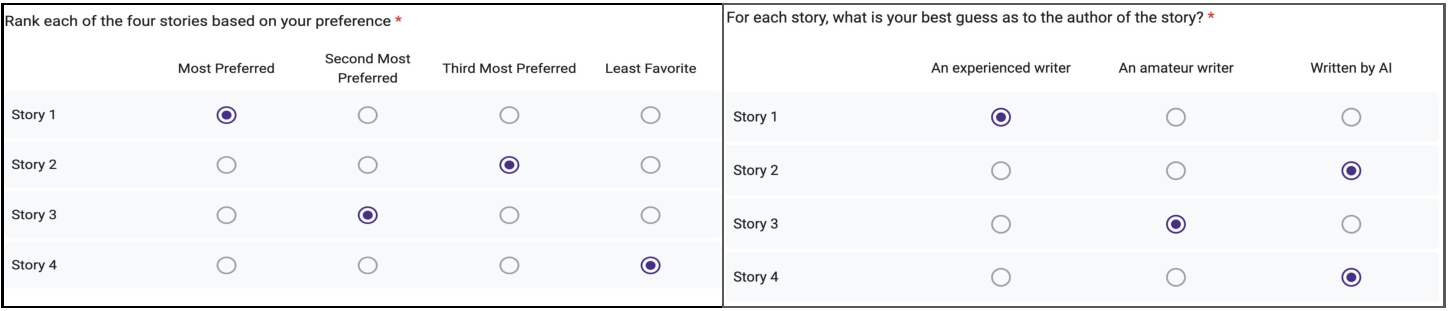
\includegraphics[width=\textwidth]{figures/rel.pdf}
    \caption{\label{relev} Relative Evaluation by Creative Writing Experts within a given cluster of four stories}
\end{figure*}
\subsubsection{Relative Evaluation with Creative Writing Experts} After providing verdict on each story inside a particular cluster we ask experts to rank the stories based on their personal preference \cite{ouyang2022training}. This evaluation was also designed with the hope that the most preferred story would also have the highest number of answers to individual questions from the absolute evaluation as `Yes'. Additionally we also ask them to guess the author of each story based on the Turing Test recommendation. We provide them 3 possible author choices to select between \textit{An expert, An amateur, AI} as can be seen in Figure \ref{relev}. This is further useful for us to study if there are certain patterns that leads experts to discriminative between model vs human written stories.